%!TEX root = ../thesis.tex
%*******************************************************************************
%****************************** Second Chapter *********************************
%*******************************************************************************

\chapter{Linear mixed models for quantitative genetics}

In chapters 4-6 I describe various models for \gls{eqtls} mapping using single cell expression profiles. 
All of these models build on a \gls{lmm} framework. 
I use this chapter to provide an overview of linear and linear mixed models and their application in quantitative genetics, with a focus on their use for e\gls{qtl} mapping. 
I will also introduce \gls{lmm}-based models to test for \gls{gxe} interactions, to provide the necessary theoretical foundations for the analyses in chapters 5 and 6.\\

\gls{lmm}s are a very popular framework for many genetic analyses. 
They are especially appealing because they provide robust control for confounding factors. 
While inference using \gls{lmm}s is in general computationally demanding, there exist efficient implementations of specific \gls{lmm}s, which enable applications to large datasets. 
In this chapter, I give an overview of the use of \gls{lmm}s in genetic association studies: in sections 2.1-2.2, I discuss the linear model (also called linear regression) and basic applications for \gls{gwas} and \gls{qtls} mapping. 
In section 2.3, I introduce the \gls{lmm} and discuss applications in genetics, with a focus on the use of \gls{lmm}s for \gls{eqtls} mapping. 
Finally, in Section 2.4, I discuss extensions of the \gls{lmm} framework to test for \gls{gxe} interactions.\\

\newpage

For mathematical model descriptions throughout this thesis, I use the following notation: bold, small letters symbolise one-dimensional column vectors (e.g. $\mathbf{v}$) and bold capitalised letters matrices (e.g. $\mathbf{M}$). 
A normal distribution is specified by $ N(\mu, \sigma^2)$, where $\mu$, $\sigma$ are two scalars representing the mean and standard deviation parameters.
For simplicity, I use the same notation for multivariate normal (e.g. $ N(\boldsymbol{\mu}, \boldsymbol{\Sigma})$), noting that the specified parameters are a Nx1 mean vector, and a NxN covariance matrix.

%********************************** %First Section  **************************************

\section{Linear regression} 

A linear model, or regression, is a statistical approach to modelling a continuous output variable (or outcome, dependent variable) as a linear function of one or more input variables (features, or independent variables). 
For F features, the outcome variable for a single individual i is:

\begin{equation} \label{eq:Linear_regression_sample_i}
 y_i = \sum_{f=1}^{F} x_{i,f}\beta_f + \psi_i
\end{equation}

The noise term $\psi_i$ ($ \psi_i \sim N(0, \sigma_n^2)$) accounts for measurement noise of $y_i$, reflecting the non-deterministic relationship between $y_i$ and $x_{i,f}$, and is assumed to follow a normal distribution with 0 mean and constant variance $\sigma_n^2$. 
Furthermore, the noise term is assumed to be independent across samples. 
For N samples, the model in \eqref{eq:Linear_regression_sample_i} can be expressed in matrix form as:

\begin{equation} \label{eq:Linear_regression_matrix_form}
\mathbf{y} = \mathbf{X}\boldsymbol{\beta} + \boldsymbol{\psi} 
\end{equation}

Where $\mathbf{y}$ is the Nx1 outcome vector, $\mathbf{X}$ is the NxF feature matrix, and $\boldsymbol{\beta}$ is the Fx1 weight vector. 
Finally, $\boldsymbol{\psi}$ is the Nx1 noise vector such that: $\boldsymbol{\psi}\sim N(\mathbf{0}, \sigma_n^2 \mathbf{I_N})$, where $\mathbf{I_N}$ denotes the NxN identity matrix. \\ 

We can then write:

\begin{equation} \label{eq:Linear_regression_MVN_form}
\mathbf{y} \sim N(\mathbf{X}\boldsymbol{\beta}, \sigma_n^2 \mathbf{I_N}) 
\end{equation}

\newpage

\subsection{Maximum likelihood solution}

Equation \eqref{eq:Linear_regression_MVN_form} is a direct representation of the probability distribution of the data $p(\mathbf{y}| \mathbf{X}, \boldsymbol{\beta}, \sigma_n^2)$ given the input variables $\mathbf{X}$ and the model parameters $\boldsymbol{\beta}$ and $\sigma_n^2$.
This probability is known as the likelihood of the model and, for parameter inference, is typically regarded as a function of the model parameters and denoted as $L(\boldsymbol{\beta}, \sigma_n^2)$. 
Thus, the model in \eqref{eq:Linear_regression_MVN_form} can be equivalently expressed as:

\begin{equation} \label{eq:Linear_regression_likelihood}
 L(\boldsymbol{\beta}, \sigma_n^2) = p(\mathbf{y}| \mathbf{X}, \boldsymbol{\beta}, \sigma_n^2) = N(\mathbf{y} | \mathbf{X}\boldsymbol{\beta}, \sigma_n^2 \mathbf{I_N}) 
\end{equation}

The log marginal likelihood ($\ell = logL$) of the model can be explicitly specified as:\\

\begin{equation} \label{eq:Linear_regression_log_likelihood}
\begin{split}
 \ell(\boldsymbol{\beta}, \sigma_n^2) = -\frac{1}{2} \bigg\{Nlog(2\pi)\sigma_n^2) + log|\mathbf{I_N}| \frac{1}{\sigma_n^2}(\mathbf{y}-\mathbf{X}\boldsymbol{\beta})^T\mathbf{I_N}^{-1}(\mathbf{y}-\mathbf{X}\boldsymbol{\beta}) \bigg\}  = \\
= -\frac{N}{2}log(2\pi)) - \frac{N}{2}log(2\pi))- 0 - \frac{1}{2\sigma_n^2}(\mathbf{y}-\mathbf{X}\beta)^T(\mathbf{y}-\mathbf{X}\beta)  
\end{split}
\end{equation}

The maximum likelihood estimator (MLE) of the model parameters is defined as the set of parameter values that maximise the likelihood (or its log). 
Denoting with $\hat{\boldsymbol{\beta}}$ and $\hat{\sigma_n^2}$ the MLE of $\boldsymbol{\beta}$ and $\sigma_n^2$ we can write:

\begin{equation} \label{eq:Linear_regression_MLEs}
\hat{\boldsymbol{\beta}},\hat{\sigma_n^2} = argmax_{\boldsymbol{\beta},\sigma_n^2}\ell(\boldsymbol{\beta}, \sigma_n^2) 
\end{equation} 

By setting the gradient of the log likelihood in \eqref{eq:Linear_regression_log_likelihood} with respect with both parameters to zero, and solving the joint system:

\begin{equation} \label{eq:Linear_regression_MLE_system}
\systeme{
    \dfrac{\partial \ell(\boldsymbol{\beta}, \sigma_n^2)}{\partial \boldsymbol{\beta}} = \mathbf{0},
    \dfrac{\partial \ell(\boldsymbol{\beta}, \sigma_n^2)}{\partial \sigma_n^2} = 0
    }
\end{equation}

We find:

\begin{equation} \label{eq:Linear_regression_MLE_solution_beta}
\hat{\boldsymbol{\beta}} = (\mathbf{X}^T\mathbf{X})^{-1}\mathbf{X}^T\mathbf{y} 
\end{equation}

\begin{equation} \label{eq:Linear_regression_MLE_solution_sigma}
 \hat{\sigma_n^2} = \frac{1}{N}(\mathbf{y}-\mathbf{X}\hat{\boldsymbol{\beta}})^T(\mathbf{y}-\mathbf{X}\hat{\boldsymbol{\beta}}) = \frac{1}{N}(\mathbf{y}-\mathbf{X}(\mathbf{X}^T\mathbf{X})^{-1}\mathbf{X}^T\mathbf{y})^T(\mathbf{y}-\mathbf{X}(\mathbf{X}^T\mathbf{X})^{-1}\mathbf{X}^T\mathbf{y}) 
\end{equation}

Note that the solution for $\hat{\boldsymbol{\beta}}$ in \eqref{eq:Linear_regression_MLE_solution_beta} is equivalent to the ordinary least squares (OLS) solution (ref).


\subsection{Restricted maximum likelihood}

In Gaussian models as in \eqref{eq:Linear_regression_MVN_form} the MLE of the variance parameter $\hat{\sigma_n^2}$ is biased because the weights $\hat{\boldsymbol{\beta}}$ are estimated from the data, which entails a reduction of the effective number of degrees of freedom.
Patterson and Thompson \cite{patterson1971recovery} proposed a solution to $\boldsymbol{\beta}$-free estimation of $\sigma_n^2$ via the restricted (or residual) maximum likelihood (REML).

Given the model in \eqref{eq:Linear_regression_matrix_form} REML can be obtained by projecting the output vector in a space that is orthogonal to $\mathbf{X}$:

\begin{equation}\label{eq:REML_0_projection}
    \mathbf{A}\mathbf{X} = \mathbf{0}
\end{equation}

Using \eqref{eq:REML_0_projection} and rewriting \eqref{eq:Linear_regression_MVN_form} in terms of the projection $\mathbf{w}$ we obtain:

\begin{equation}\label{eq:REML_w_projection}
    \mathbf{w} = \mathbf{A}\mathbf{y} = \mathbf{A}(\mathbf{X}\boldsymbol{\beta} + \boldsymbol{\psi}) = \mathbf{A}\boldsymbol{\psi}
\end{equation}

which provides an expression of $\mathbf{y}$ that is independent of $\boldsymbol{\beta}$.\\

By estimating $\ell(\sigma_n^2 | \mathbf{A}\mathbf{y} )$ for the model in \eqref{eq:Linear_regression_log_likelihood}, we obtain the following log restricted maximum likelihood:

\begin{equation} \label{eq:Linear_regression_log_restricted_likelihood}
\begin{split}
\ell(\sigma_n^2) = -\frac{N-F}{2}log(2\pi) - \frac{1}{2}log|\mathbf{X}^T\mathbf{X}| \\
-  \frac{N-F}{2}log\sigma_n^2 - \frac{1}{2\sigma_n^2}(\mathbf{y}-\mathbf{X}\hat{\boldsymbol{\beta}})^T(\mathbf{y}-\mathbf{X}\hat{\boldsymbol{\beta}})  
\end{split}
\end{equation}

which is maximised by

\begin{equation}\label{eq:Linear_regression_REML_sigma}
\hat{\sigma_n^2}_{REML} =  \frac{1}{N-F}(\mathbf{y}-\mathbf{X}(\mathbf{X}^T\mathbf{X})^{-1}\mathbf{X}^T\mathbf{y})^T(\mathbf{y}-\mathbf{X}(\mathbf{X}^T\mathbf{X})^{-1}\mathbf{X}^T\mathbf{y})
\end{equation}

Note that \eqref{eq:Linear_regression_REML_sigma} is identical to \eqref{eq:Linear_regression_MLE_solution_sigma} with the exception that N is replaced by (N - F), which denotes the loss of F degrees of freedom.

%********************************** %Second Section  **************************************

\section{Linear models for association studies}

When applying linear models in genetic association studies, the outcome variable ($\mathbf{y}$) is a phenotype, which is a measurable characteristic of the samples considered. 
In \gls{gwas}, we typically look at "global phenotypes".
These can be traits such as height and eye colour or disease status/risk for various illnesses (such as diabetes, or rheumatoid arthritis, see Section 1.1.y).
In \gls{qtl} mapping, we consider "molecular phenotypes". 
Those can be quantification of molecular traits such as gene expression (i.e. e\gls{qtl}), or protein level (p\gls{qtl}), etc. (Section 1.2.x).
The test then consists in assessing the effect of single nucleotide polymorphisms (SNPs),  onto such phenotype. 
We test the effect of one SNP ($\mathbf{g}$) at a time, onto such phenotype:

\begin{equation}\label{eq:Linear_regression_genetics}
 \mathbf{y} = \mathbf{g}\beta + \boldsymbol{\psi} 
\end{equation}

We assume all SNPs to be biallelic, that is that they can only assume two possible values. 
Let us consider a bi-allelic variant with major allele a and minor allele A. For the minor allele A, we can consider either a dominant model (aa = 0, Aa = 1, AA = 1; where only one copy of the allele is necessary to have a phenotypic effect), a recessive model, (aa = 0, Aa = 0, AA = 1; where two copies of the minor allele must be present for a phenotypic effect) or an additive model (aa = 0, Aa = 1, AA = 2; where the effect is proportional to the minor allele count). 
In this thesis, we will consider an additive genetic model, which is widely-used in the analysis of complex traits (ref).

\subsection{Traits with binary outcomes}

It is worth noting that linear regressions are well suited for continuous traits, which can be approximated to follow a normal distribution. 
Another widely used model for genetic analyses is the logistic regression (or logit regression), where a logit function is applied to a linear predictor ($\mathbf{z}$) to better reflect the data in case of binary outcomes ($\mathbf{y}$). 
This is very often used when the phenotype of interest reflects the presence or absence of a certain disease - the so called case/control studies.
In this case, the outcome can be thought of in terms of sampling from a binomial distribution, with a fixed number of samples N, and a probability p to have the disease. Then, the model becomes:

\begin{equation}\label{eq:Logistic_regression_genetics_z}
 logit(\mathbf{y}) = \mathbf{z} = \mathbf{g}\beta + \boldsymbol{\psi} 
\end{equation}

Logistic regressions are a particular example of a larger class of models, the generalised linear models (GLMs). 
GLMs are used when the distribution of the outcome variable cannot be approximated to a Gaussian distribution. 
In the example above, a logit distribution is better suited to model a binary variable. 
In other cases, we might have count data better approximated by a Poisson distribution, etc.
The three requirements of a GLM are i) to have a linear predictor ($\mathbf{z}$), ii) that the distribution of $\mathbf{y}$  belongs to the exponential family (Box\ref{box3}), and iii) that we can define a link function $g$ such that:

\begin{equation*}
 E[\mathbf{y}] = g(\mathbf{z})^{-1} 
\end{equation*}

In \eqref{eq:Logistic_regression_genetics_z}, $ g = logit $.


%****** Box on exponential family distributions ******

\newpage

\begin{Comment}
\hspace{-2.5mm}\textbf{Box 3: Exponential Family distributions}\label{box3}\\
% \small
In probability and statistics, an exponential family is a parametric set of probability distributions of the form:

\begin{equation*}
    p(x) = h(x)e^{\theta^TT(x)-A(\theta)}
\end{equation*}

Members of the exponential family distributions include:
\begin{itemize}
    \item Normal distribution: $X \sim N(\mu,\sigma^2)$
    \item Exponential distribution: $ X \sim Exp(\lambda)$
    \item Gamma distribution: $ X \sim \Gamma(\alpha,\beta)$
    \item Chi-squared distribution: $ X \sim \chi^2 (k)$ or $ X \sim \chi_k^2$
    \item Beta distribution: $ X \sim Beta(\alpha,\beta)$
    \item Dirichlet distribution: $ X \sim Dir(\alpha)$
    \item Bernoulli distribution: $ X \sim Be(p)$ or $ X \sim Bernoulli(p)$
    \item Poisson distribution: $ X \sim P(\lambda)$ or $ X \sim Pois(\lambda)$
    \item Binomial distribution (with fixed number of trials): $ X \sim B(n,p)$
    \item Negative Binomial distribution (with fixed number of failures): $ X \sim NB(r,p)$\\
\end{itemize}

For example, take the Bernoulli case: $x \in X \sim Be(p)$:

\begin{equation*}
\begin{split}
    p(x) & = p^x(1-p)^{(1-x)}\\
         & = e^{log(p^x(1-p)^{(1-x)})}\\
         & = e^{xlogp + (1-x)log(1-p)}\\
         & = e^{xlog\frac{p}{1-p}+log(1-p)}\\
         & = e^{x\theta - log(1+e^\theta)}
\end{split}
\end{equation*}

where: 

\hfill $h(x)=1 \hfill T(x)=x \hfill \theta = log \frac{p}{1-p} \hfill A(\theta) = log(1+e^\theta)$ \hfill

\end{Comment}

%**************

\newpage

\subsection{Statistical hypothesis testing}

To test for whether an association between a genetic variant and a trait is present, we can compare the hypothesis where the genetic variant has no effect on the trait (called null hypothesis, $H_0$) and the alternative hypothesis when the variant does have an effect (effect different from 0, $H_1$).
Formally, the association hypothesis test is:

\begin{equation}\label{eq:null_hypothesis}
 H_{0}: \beta=0 
\end{equation}
vs
\begin{equation}\label{eq:alternative_hypothesis}
 H_{1}: \beta \neq 0 
\end{equation}

We are then comparing the following models (from \eqref{eq:Linear_regression_genetics}):

\begin{equation}\label{eq16:null_hypothesis_regression}
 H_0: \mathbf{y} \sim N(\mathbf{0}, \sigma_n^{2} \mathbf{I_N}) 
\end{equation}

\begin{equation}\label{eq17:alternative_hypothesis_regression}
 H_1: \mathbf{y} \sim N(\mathbf{g}\beta,\sigma_n^{2} \mathbf{I_N}) 
\end{equation}

Statistical hypothesis testing consists of three fundamental steps: i) define a test statistic; ii) obtain a P-value and iii) upon a threshold on the P-value, reject or accept the null hypothesis. 
A test statistic is a random variable that quantifies the difference between the null hypothesis $H_0$ and what is observed in the sample. 
Once we have a test statistic, we calculate a probability value ("p value") as the probability, under the null hypothesis $H_0$, of sampling a test statistic at least as extreme as the observed one. 
An extreme value of the test statistic generally indicates evidence against $H_0$.
The p value is a function of the test statistic and, by definition, it is uniformly distributed under $H_0$.
Finally, if this probability is low (under a defined threshold, e.g. P < 0.05) $H_0$ is rejected and $H_1$ accepted (positive result).
Otherwise, we reject $H_1$ and accept $H_0$ (negative result).\\

In statistical hypothesis testing, two types of errors can be made. 
We can either reject $H_0$ when $H_0$ is true, thus generating a false positive (type I error), or reject $H_1$ when $H_1$ is true, generating a false negative (type II error).
Other concepts that are central to statistical hypothesis testing are the significance level, defined as the type I error rate (i.e. the expected percentage of false positives), and the statistical power, which is the true positive rate under $H_1$ (i.e. the ability to recover true associations, Box\ref{box4}).

%****** Box on confusion matrix ******

\newpage

\begin{Comment}
\hspace{-2.5mm}\textbf{Box 4: Key concepts of statistical testing}\label{box4}\\
% \small
Confusion matrix:

\begin{center}
\begin{tabular}{l|l|c|c|}
\multicolumn{2}{c}{}&\multicolumn{2}{c}{Test Result}\\
\cline{3-4}
\multicolumn{2}{c|}{}&reject $H_0$&accept $H_0$\\
\cline{2-4}
\multirow{2}{*}{Actual value}& $H_1$ & True Positive ($TP$) & False Negative ($FN$)\\
\cline{2-4}
& $H_0$ & False Positive ($FP$) & True Negative ($TN$)\\
\cline{2-4}
\end{tabular}
\end{center}

\begin{itemize}
    \item Type I error $= FP$
    \item Type II error $= FN$
    \item Sensitivity $=$ Recall $=$ True positive rate (TPR) $=$ Power $=\frac{TP}{TP+FN}$
    \item Specificity $=$ True negative rate (TNR) $=\frac{TN}{TN+FP}$
    \item False positive rate (FPR) $= 1-$Specificity $=$ Size $=\frac{FP}{TN+FP}$
    \item Precision $=$ Positive predictive value (PPV) $=\frac{TP}{TP+FP}$
    \item Accuracy $=\frac{TP+TN}{TP+TN+FP+FN}$
    \item $F_1$ score $F_1=2 \frac{PPV*TPR}{PPV+TPR}=\frac{2TP}{2TP+FP+FN}$
    \item Family-wise error rate (FWER) $=P(FP \geq 1)= 1 - P(FP=0)$
    \item False discovery rate (FDR) $=\frac{FP}{TP+FP}= 1- $Precision
\end{itemize}

\vfill

\end{Comment}

%**************

\vspace{5mm}

Three approaches are commonly used for statistical testing in genetic association analyses: the Wald test, the \gls{lrt}, and the score test     (Fig. \ref{fig:hypothesis_tests}).
In the next paragraphs, I will describe briefly all three but note that only the two latter are used in this thesis.

\begin{figure}[h]
\centering
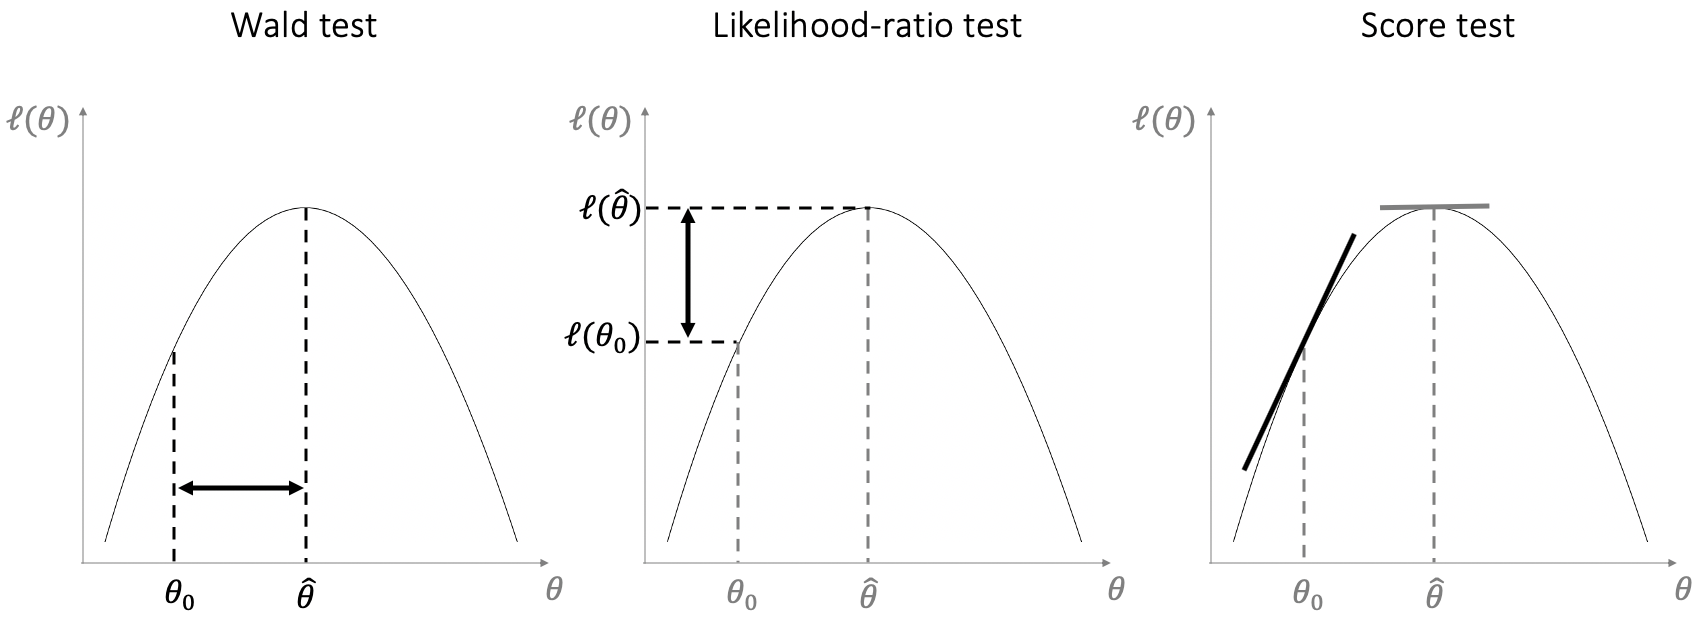
\includegraphics[width=15cm]{Chapter2/Fig/wald_lrt_score_tests.png}
\caption[\textbf{Wald, LRT and score test}]{\textbf{The Wald test, the likelihood-ratio test and the score test}.\\
The three most commonly used statistical testing approaches are illustrated here in the univariate case (single parameter $\theta$). 
On the x axis is the parameter $\theta$ on the y axis the log likelihood $\ell(\theta)$.
The Wald test essentially evaluates the difference between the MLE $\hat{\theta}$ and the parameter under $H_0$, $\theta_0$.
The likelihood-ratio test evaluates the difference between the log likelihoods evaluated at those values, i.e. $\ell(\hat{\theta})$ and $\ell(\theta_0)$.
Finally, the Score test evaluates the slope of $\ell(\theta)$ at $\theta_0$. Note that the slope at $\hat{\theta}=0$ by definition, as the MLE maximises $\ell(\theta)$.}
\label{fig:hypothesis_tests}
\end{figure}

\subsubsection{Wald test}

First, let us consider the Wald test and the generic null hypothesis $H_0: \boldsymbol{\theta} = \boldsymbol{\theta}_0$ and the alternative $H_1: \boldsymbol{\theta} \neq \boldsymbol{\theta}_0$.
The Wald test statistic is defined as:

\begin{equation}\label{eq:Wald_test}
W = (\hat{\boldsymbol{\theta}}-\boldsymbol{\theta_0})^T [var(\boldsymbol{\theta_0})]^{-1}(\hat{\boldsymbol{\theta}}-\boldsymbol{\theta_0}) 
\end{equation}

Under some assumptions (ref), $W$ follows a chi-squared ($\chi^2$) distribution with number of degrees of freedom (dof) $d$ equal to the number of tested parameters ($W \sim \chi^2_d $).\\

In the univariate case (d = 1), \eqref{eq:Wald_test} can be expressed as:

\begin{equation}\label{eq:Wald_test_univariate}
    W = \frac{(\hat{\theta}-\theta_0)^2}{var(\hat{\theta})} \sim \chi^2_1
\end{equation}

Intuitively, the chance of rejecting $H_0$ increases as $\hat{\theta}$ is further away from $\theta_0$
and decreases as our confidence in the estimation of the MLE (i.e. $var(\hat{\theta})$) increases.


\subsubsection{Likelihood ratio test}

The second test we consider is the \gls{lrt}.
% It was first introduced by XX. 
The test statistic in this case is the (log) likelihood ratio ($LLR$):

\begin{equation}\label{eq:log_likelihood_ratio}
LLR = log \frac{L(H_1)}{L(H_0)} = \ell(H_1) - \ell(H_0) 
\end{equation}

Where we compare the value of the log-likelihood of the model under $H_0$ and $H_1$, by evaluating \eqref{eq:Linear_regression_log_likelihood} (or \eqref{eq:Linear_regression_log_restricted_likelihood}) using MLE parameters estimated under $H_0$ ($\mathbf{0}$, $\sigma_0^2$) or $H_1$ ($\hat{\boldsymbol{\beta}}$, $\hat{\sigma_1^2}$).  \\

The Wilks theorem (1938), under some assumptions, guarantees that $2LLR$, too, follows a $\chi^2$ distribution with $d$ dof ($2LLR \sim \chi^2_d$).

The P-value can then be calculated as:

\begin{equation}\label{eq:lrt_p_value}
    P(LLR) = 1-F_{\chi^2}(2LLR; d)
\end{equation}

\subsubsection{Score test}

Finally the score test, also known as Lagrange multiplier test, is the last hypothesis test we consider. 
It was first developed by Rao in 1948 (\cite{rao1948large}).
First, we define the score vector of Fisher as the gradient of the likelihood with respect to its parameters:

\begin{equation}\label{eq:score_vector}
    \mathbf{S} = \frac{\partial L}{\partial \boldsymbol{\theta}}
\end{equation}

The Score test statistic is the Lagrange Multiplier (LM) and is defined as follows:

\begin{equation}\label{eq:lagrange_multiplier}
    LM = \mathbf{S}(\boldsymbol{\theta_0})^T [var(\boldsymbol{\theta_0})]^{-1}\mathbf{S}(\boldsymbol{\theta_0}) 
\end{equation}

It can be shown that $LM$, too, follows a $\chi^2$ distribution with $d$ dof ($LM \sim \chi^2_d$).

To understand the intuition behind this test let us consider again the univariate case (d = 1):

\begin{equation}\label{eq:lagrange_multiplier_univariate}
    LM = \frac{S(\theta_0)^2}{var(\theta_0)} \sim \chi^2_1
\end{equation}

At the MLE $\hat{\theta}$, the log likelihood and therefore its gradient $S(\hat{\theta})$ is equal to 0.
On the contrary, in principle, $ S(\theta_0) \neq 0 $ (Fig. \ref{fig:hypothesis_tests}). 
Intuitively, the further away from 0, the more likely we are to reject the null hypothesis.
Fast methods to infer the p-value of a Score test were proposed by Davies  \cite{davies1980algorithm} and Liu (ref).

% Davies exact method and Liu:

% \begin{equation}
%     P(Q<c)
% \end{equation}


\subsubsection{Intuition on differences between LRT and score test}

In this thesis, we apply both the \gls{lrt} and the Score test, for different applications.
I use this paragraph to highlight the key differences between the two tests and provide an intuition as to when one should use one or the other.\\

First of all, it can be shown that (finite sample, ref):

\begin{equation}\label{eq:W_LLR_LM}
    W \geq LLR \geq LM
\end{equation}

Let us exclude the Wald test for this purposes, \eqref{eq:W_LLR_LM} guarantees that the log-likelihood ratio is always greater than the Lagrange multiplier.
As a consequence, the power (Box\ref{box4}) of the \gls{lrt}, defined as the probability of rejecting the null hypothesis when it is false: $P = P($reject $H_0 | H_1)$ is higher than the power of the Score test.

\begin{equation}
    (P_W \geq) P_{LLR} \geq P_{LM}
\end{equation}

On the other hand, the false positive rate (FPR, Box\ref{box4}) of the \gls{lrt}, defined as the probability of rejecting the null hypothesis when it is true: FPR $= P($reject $H_0 | H_0)$ is also higher than the FPR of the Score test.
The Score test is therefore more accurate, making a smaller (or equal) number of Type I errors. The \gls{lrt} is robust to re-parametrization of the parameters, whereas the score test (or the Wald test) is not. On the other hand, one main advantage of the Score test is that it does not require the evaluation of the MLE of the parameters, but only evaluate the likelihood under the null hypothesis.
Finally, the LLR follows a $\chi^2$ distribution (asymptotically) only under the assumptions of the Wilks' theorem, which can be violated in certain applications.
Namely, the value of parameters tested should be far away from the boundaries of the possible values the parameter can assume.
For example, $-\infty < \beta < \infty$, so testing $H_1: \beta \neq 0$ satisfies the assumption.
On the other hand, $0 < \sigma^2 < \infty$ so testing $H_1: \sigma^2 \neq 0$ violates the assumption, because the value $0$ is right at the boundary.\\

I will use the \gls{lrt} in the analyses in chapters 4 and 5, where the tests evaluate $\beta$.
I use Rao's score test in chapter 6, where I will be evaluating the variance parameter $\sigma^2$.


\subsection{Multiple Testing Correction}

Hundreds of thousands or millions of variants may be individually tested within a typical human \gls{gwas}. 
In e\gls{qtl} mapping, we might test tens of thousands of genes, each essentially equivalent to a \gls{gwas} trait. 
Even when we only test for \textit{cis} e\gls{qtl}, we will still test hundreds of variants per gene, bringing the average number of tests performed well in the Millions (ref).  
When performing such a large number of tests, controlling single test p values results in a high number of false positives (for example, for P < 0.01 and 10$^6$ tests we expect 10,000 false positives under the null hypothesis). 
This problem is known as the multiple hypothesis testing problem. 
In the next paragraphs, I give a brief overview of the methods commonly used in genetic analysis to correct for multiple hypothesis testing, with a focus on methods used in e\gls{qtl} mapping.

\subsubsection{Controlling family-wise error rate} 

One strategy to perform multiple testing correction is to control the probability of having at least one false positive for a trait, which corresponds to a trait-wise p value known as family-wise error rate (FWER, Box\ref{box4}).
The widely used Bonferroni method follows this strategy assuming independence between tests. 
Given a desired family-wise significance level $\alpha$, the method consists in calculating adjusted p values as $P_{adj} = P*n $, where n is the number of tests, and setting $P_{adj} < \alpha$ . 
This strategy ensures FWER < $\alpha$. 
The Bonferroni correction strategy is conservative, because of the assumption of independence between tests, which ignores correlations between genotypes due to linkage disequilibrium (LD).\\

An alternative strategy, which accounts for the dependency of the statistical tests, is to consider permutations. 
For example, one way to control the FWER by using permutations is to perform the association test with a trait M times, each time considering a different permutation of the genotype data across individuals.
The minimum p values from these M additional experiments are then used to calculate a trait-wise p value, as the fraction of the M minimum permutation p values that are lower than the minimum observed p value. 

For test i, the experimental adjusted p value after M permutations is calculated as:

\begin{equation}\label{eq:permutation_adjusted_pvalue}
    P_{adj,i}^{perm} = \frac{1+\sum_{m=1}^{M} q_{i,m} \geq P_i}{1+M}
\end{equation}

Where $q_{i,m}$ is the p value obtained at the m$^{th}$ permutation run equivalent to test i, and ones are added to avoid zero divisions.  
This strategy accounts for local LD, thereby increasing the statistical power, and has been widely used in $cis$ molecular \gls{qtl} mapping to estimate gene-level p values \cite{gtex2015genotype}.  

% rephrase this
Second, significant p values are truncated to a limited level of significance determined by the number of permutations. For example, 10,000 permutations restrict the p values to a lower bound of $10^{-4}$. Typically, one will obtain a list of genes that have the same lower-bound p values, such as $10^{-4}$. However, it is desirable to know the exact significance of each eGene p value for better interpretation and prioritization of genes.

However, as evident from \eqref{eq:permutation_adjusted_pvalue}, a potentially very large number of permutations is needed to be able to detect a range of effects, as significant p values using this method are truncated.
For example for M=1,000 the smallest adjusted p value we can obtain is only $P_{adj}$=0.001 (when no permuted p value is smaller than the p value observed); for M=10,000 the lower-bound p-values will be $10^{-4}$. 
Typically, one will obtain a list of genes that have the same lower-bound p values, such as $10^{-4}$. 
However, it is desirable to know the exact significance of each eGene p value for better interpretation and prioritization of genes \cite{sul2015accurate}.
This can be improved by increasing the number of permutations, e.g. using M as large as 100,000, but that entails a great computational burden and can become unpractical in molecular analyses of large cohorts.\\

Recently, one method has been developed that uses permutation results for as little as (M=) 50-100 permutations to estimate a full distribution of background permuted p values, allowing to exploit the benefits of the assumption-free permutation approach without too much of the computational burden \cite{ongen2016fast}. 
This is the method I will use throughout this thesis to control for FWER at gene level when performing large scale e\gls{qtl} mapping.

\subsubsection{Controlling false discovery rate}

An alternative solution is to control the false discovery rate (FDR), i.e. the expected percentage of false discoveries (Box\ref{box4}).
The most widely used FDR-based correction method is the Benjamini-Hochberg (BH) procedure \cite{benjamini1995controlling}, which again assumes independence between tests. 
Let us consider T tests with p values $p_1, p_2, ..., p_T$ and let $r_1, r_2, ..., r_T$ be their ranks (the smallest p value has rank 1, the highest has rank T), defining adjusted p values as $P_{adj,i} = \frac{T*p_i}{r_i} $ and setting $P_{adj,i} <\alpha$ ensures FDR < $\alpha$.
More recently, the Storey procedure \cite{storey2002direct} optimises the BH procedure by taking into account the distribution of the p values in the experiment.
FDR corrected p values using the Storey procedure are sometimes called 'q-values'.\\

% add intuition behind FWER/FDR?

For e\gls{qtl} mapping, the assumption of independent tests holds when we only consider the top SNP per gene.
In this case, the number of tests T coincides with the numbers of genes tested.
Conditional analyses (where we include the top SNP as a covariate in the model) can be used subsequently to detect secondary and tertiary effects for a gene.

\subsubsection{Multiple testing correction for \textit{cis} e\gls{qtl} mapping}

A typical strategy to correct for multiple hypothesis testing in molecular \textit{cis}-\gls{qtl} mapping is to use a two-step procedure \cite{gtex2015genotype} (refs). 
First, for each gene an experiment-wise p value is obtained by correcting for multiple testing across variants using a FWER-based method. 
These gene-level p values are probability values for the hypothesis of a gene having at least
one e\gls{qtl} in the analysed region. 
Second, the gene-level p values are corrected to control the FDR, using either the Benjamini-Hochberg or the Storey procedure.\\

In the analyses in Chapters 4 and 5 of this thesis, I adopt this two step approach.
I use M=1,000 permutations and the method described in \cite{ongen2016fast} to correct p values at the gene level (I will call the p values obtained this way "empirical feature p values").
Then, I select the top SNP per gene and correct the corresponding empirical feature p values a second time, using the Storey procedure \cite{storey2002direct}.
I will call the resulting P-values: "globally corrected p values".

\subsection{Confounding effects in linear model}

The model in \eqref{eq:Linear_regression_genetics} only models the SNP tested as a factor affecting the measured phenotype.
However, if available, additional relevant information for the samples tested (such as sex or age) can be added to the model as covariates $\mathbf{W}$ and often improve the model:

\begin{equation}\label{eq:Linear_regression_genetics_covariates}
 \mathbf{y} =  \mathbf{W}\boldsymbol{\alpha} + \mathbf{g}\beta + \boldsymbol{\psi} 
\end{equation}

Those covariates are implemented as fixed effects (FEs), and they only contribute to the mean value of $\mathbf{y}$, such that $E[\mathbf{y}] = \mathbf{W}\boldsymbol{\alpha} + \mathbf{g}\beta$, while $Cov(\mathbf{y}) = Cov(\boldsymbol{\psi}) = \sigma_n^2 \mathbf{I_N} $, as before.
In some cases, we can add fixed effect covariates for other confounding, such as technical batches and other experimental conditions that might skew the results. \\

In e\gls{qtl} mapping, we can often take advantage of the expression profiles across all genes to identify global confounding affecting the expression of genes, even when we do not necessarily know the origin of the confounding.
For example, we can compute principal component analysis (PCA) on the full expression matrix (genes x samples) and include the first 5, 10, 20 or 50 PCs as covariates in the model.
Alternative more sophisticated methods to compute factors capturing global trends are probabilistic estimation of expression residuals (PEER) \cite{stegle2010bayesian, stegle2012using} and multi-omics factor analysis (MOFA) \cite{argelaguet2018multi}. 

\subsection{Calibration studies and distributions on P-values}

Under the assumption of no association between genetic variants and the analysed trait, an association model is expected to produce approximately uniform p values.
If that is the case, the model is said to be calibrated.
To verify that a model is calibrated we can disrupt the association between genotypes and phenotypes, by shuffling the genotypes. 
A representation that is often used to compare the observed (shuffled) and the expected distributions of p values is the quantile-quantile plot (QQ plot). 
In a QQ plot the observed -log10P is plotted against the expected -log10P, where the expected value is obtained from the uniform distribution. 
As confounding factors may create spurious associations, inflated QQ plots are typically associated with the presence of confounding and can be used as a diagnostic tool (Fig. \ref{fig:qqplots}). 

\begin{figure}[h]
\centering
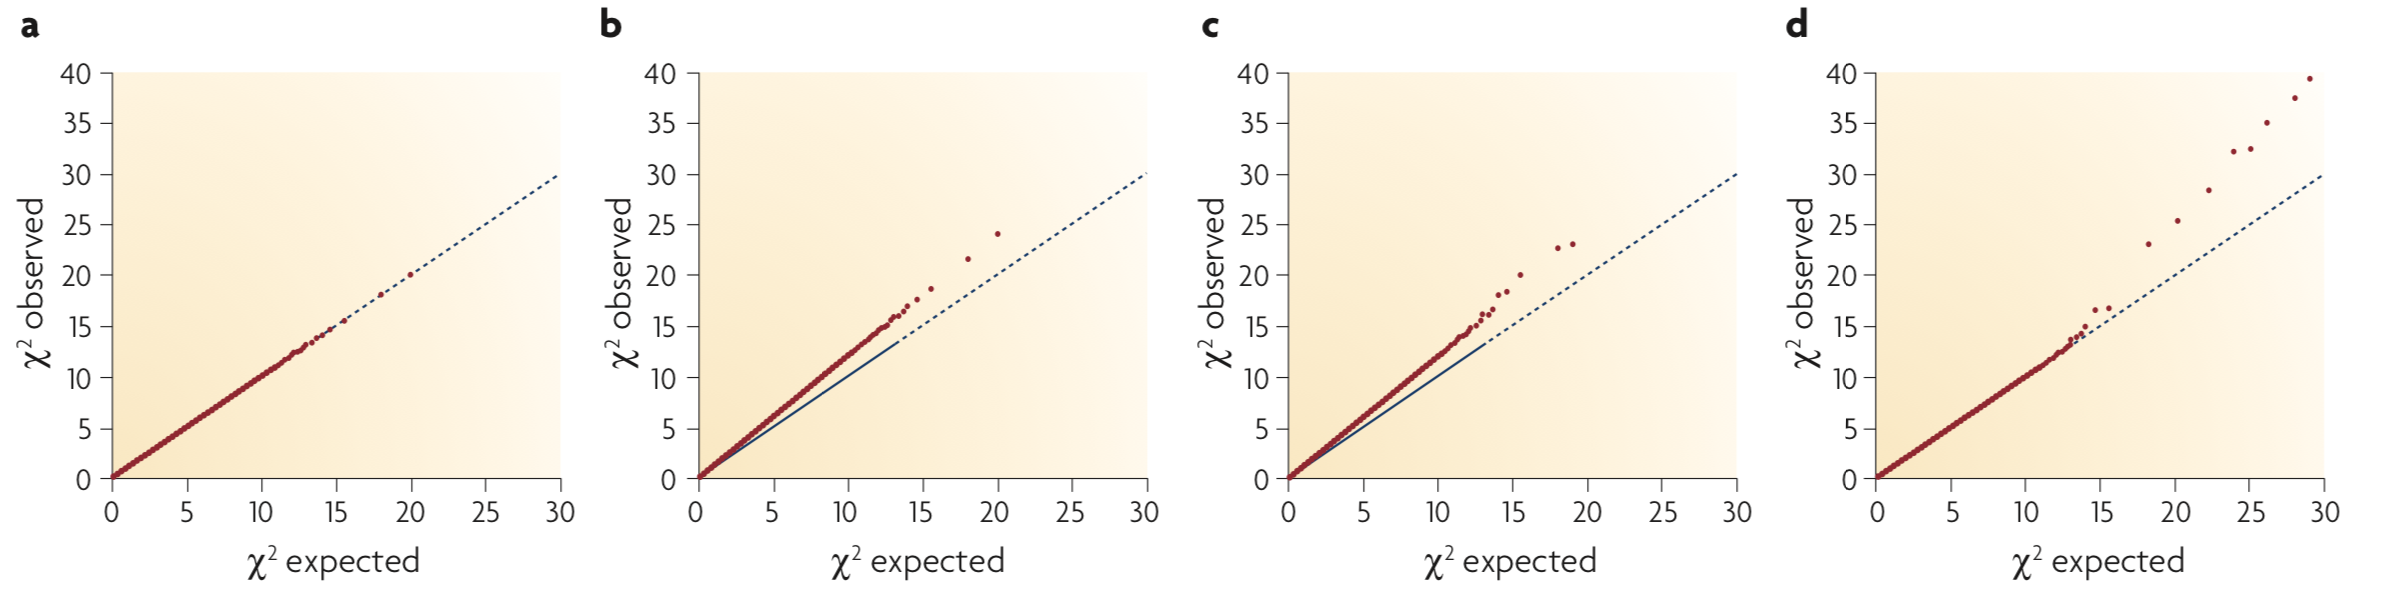
\includegraphics[width=15cm]{Chapter2/Fig/qqplots.png}
\caption[\textbf{QQplots}]{\textbf{QQplots}.\\
Placeholder adapted from McCarthy \textit{et al}, 2008
(a) no association (b) cryptic relatedness (c) population stratification (d) genuine association}
\label{fig:qqplots}
\end{figure}


%********************************** %Third Section  **************************************

\section{Population structure and linear mixed models}

One major source of confounding effects in genetic analysis - that I have purposefully left out so far -  is latent population substructure, which includes population stratification (the presence in study samples of individuals with different ancestral and demographic histories) and cryptic relatedness (evidence that individuals in the study sample have residual, non-trivial degrees of relatedness) \cite{mccarthy2008genome}.
It was acknowledged, even before the first \gls{gwas} was conducted, that there was a possibility of identifying false positives (or that true positives may be masked) when using population based association studies (instead of family based linkage studies), due to those confounding effects (ref). 
This is because both phenotypic prevalence (proportion of individuals exhibiting the phenotype) and allele frequencies (frequencies of a specific allele within a population) vary across different populations, which may result in the identification of spurious association between variants and the phenotype of interest due to ethnicity or population sub-structure (ref).

% name examples

\subsection{Approaches to account for population structure}

Various approaches have been proposed:
For example, a method that attempts to correct the underlying problem is STRUCTURE, which assigns individuals to discrete populations subgroups and then combines the evidence for association across the different subgroups \cite{pritchard2000inference}. 
However, this method does not scale with sample size and is also highly sensitive to the number of defined population clusters.\\

Ideally, if we knew the underlying sub-population structure of our samples and therefore which variants showed different allele frequencies between such groups, we could simply include such variants as covariates (i.e. similar to $\mathbf{W}$ from \eqref{eq:Linear_regression_genetics_covariates}:

\begin{equation}
    \mathbf{y} =  \mathbf{W}\boldsymbol{\alpha} +  \mathbf{G}_{conf}\mathbf{b}_{conf} + \mathbf{g}\beta + \boldsymbol{\psi} 
\end{equation}

However, this is not typically the case.
Furthermore, the number of variants might be rather large.
Instead, we can attempt to capture the main genotypic sources of variation by performing PCA on the full genotype matrix NxM $\mathbf{G}$, where M is the number of SNPs \cite{price2006principal}.
Then, we can include the first p PCs as covariates, where p is typically determined as the number of PCs that cumulatively describe a certain proportion of the total variance (ref):

\begin{equation}
    \mathbf{y} =  \mathbf{W}\boldsymbol{\alpha} + \sum_{i=1}^{p} PC_i b_i + \mathbf{g}\beta + \boldsymbol{\psi} 
\end{equation}

This approach was shown to perform relatively well in removing global population structure, but often failed to detect subtle relatedness effects (ref).\\

Linear mixed models (\gls{lmm}s) can be used to successfully account for confounding linked to latent population structure.
The intuition is to consider eq (2.32), but this time considering SNPs from the whole genome, since we do not know the "confounding variants" ($\mathbf{y} =  \mathbf{W}\boldsymbol{\alpha} +  \mathbf{G}\mathbf{b} + \mathbf{g}\beta + \boldsymbol{\psi}$).
Now, if we assume that the weights $\mathbf{b}$ come from a normal distribution $\mathbf{b} \sim N(\mathbf{0},\sigma^2_g\mathbf{I_M})$, where $M$ is the total number of SNPs.
It can be shown that:

\begin{equation}
    \mathbf{u} =  \mathbf{G}\mathbf{b} \sim N(\mathbf{0},\sigma^2_g \mathbf{G}\mathbf{G}^T)
\end{equation}

Where $\mathbf{u}$ is a random variable which captures the effect of latent population structure onto $\mathbf{y}$.
The model we just described is a \gls{lmm}.\\

In terms of removing effects of population stratification, \gls{lmm}s have been shown to perform exactly as well as  including all M PCs (or regressing them out, ref), which is of course not feasible in practice.
Additionally, it successfully corrects for more subtle effects due to cryptic relatedness.
However, \gls{lmm}s are typically much more computationally demanding.
The next section describes \gls{lmm}s in general and introduces fast implementation approaches for a specific class of \gls{lmm}s.

\subsection{Linear mixed models}

In a linear mixed model (\gls{lmm}) the outcome variable can be described by a sum of deterministic effects (fixed effects, FE) and random effects (RE).
A random effect is ..
A \gls{lmm} can be expressed as:

\begin{equation}\label{eq:Linear_mixed_model}
 \mathbf{y} =  \mathbf{W}\boldsymbol{\alpha} + \mathbf{Z}\mathbf{b} + \boldsymbol{\psi} 
\end{equation}

Where $\mathbf{y}$ is the outcome variable, $\mathbf{W}$ and $\mathbf{Z}$ are the design matrix of fixed and random effects respectively; $\boldsymbol{\alpha}$ are the fixed effects, $\mathbf{b} \sim N(\mathbf{0},\sigma_b^2\boldsymbol{\Sigma_b})$, $\boldsymbol{\Sigma_b}$ is a known covariance matrix, $\boldsymbol{\psi} \sim N(\mathbf{0},\sigma_n^2\mathbf{I})$ is the noise vector and $\sigma_b^2$ and $\sigma_n^2$ are the variance parameters of the random effect and the noise, respectively.\\

Differently from the case of linear regression discussed in \textbf{Section 2.1}, there is no close-form solution for the (restricted) MLE of the model parameters. \\

However, for the model in eq (2.34) it is possible to speed up computations, provided that we can perform feature selection on genomic variants and therefore make the genetic relatedness matrix low rank (ref): 

\begin{equation}\label{eq22:Linear_mixed_model}
 \mathbf{y} =  \mathbf{W}\boldsymbol{\alpha} + \mathbf{g}\beta + \mathbf{u} + \boldsymbol{\psi} 
\end{equation}


$\mathbf{u} \sim N(\mathbf{0}, \sigma_g^2\mathbf{K})$\\


Note that for ease of notation in the following equations I will drop the subscript $N$ from the identity matrix (i.e. $\mathbf{I} = \mathbf{I}_N$):

\begin{equation}\label{eq34}
 \mathbf{y} \sim  N(\mathbf{W}\boldsymbol{\alpha} + \mathbf{g}\beta, \sigma_g^2\mathbf{K} + \sigma_n^2\mathbf{I})
\end{equation}

Where $\mathbf{K}$ can be the genetic relatedness matrix:

\begin{equation}
    GRM = \frac{1}{M}\mathbf{G}\mathbf{G}^T
\end{equation}

% As I will show in Section 2.3.3, an efficient derivative-free inference scheme can be used for association testing in univariate models 
% % \cite{}. 
% However, the number of variance parameters in variance component analyses and multi-trait models is typically too large for the efficient use of derivative-fee methods. 

% Multiple optimisation schemes have been proposed to optimise the restricted marginal likelihood in these cases


% FaST-LMM, BOLT-LMM, LIMIX.

% , including first-derivative methods, such as expectation maximisation (EM, Dempster et al., 1977) and its improved version PX-EM (Liu et al., 1998; Foulley and Van Dyk, 2000), and second-derivative methods, such as the Newton-Ralphson algorithm (Zhou and Stephens, 2014), the average information REML algorithm (Gilmour et al., 1995) and the Broyden’s method (Groeneveld, 1994). In this thesis, we follow (Groeneveld, 1994) and consider the Broyden’s method for parameters inference. 

% For a discussion on the different optimisation algorithms for inference in \gls{lmm}s, I refer to the supplementary information of Loh et al. (2015a).

In this thesis, we employ the approach first proposed by Lippert et al. \cite{lippert2014limix} and which is implemented within the LIMIX toolset \cite{lippert2014limix,casale2015efficient}. 
Briefly, \cite{lippert2014limix} compute the eigenvalue decomposition of the genetic kinship matrix $\mathbf{K}$ once, and then use the decomposition to project all data into a space where phenotypic variables and covariates are uncorrelated. 
This transformed data can then be subjected to standard association analyses \cite{lippert2014limix}.

\subsection{Fast \gls{lmm}s for e\gls{qtl} mapping}





% GRM: genetic relatedness matrix

% IBD: identical by descent

% plink (Purcell)

To account for population stratification and relatedness (ref)

Fast\gls{lmm} tricks:
\begin{itemize}
    \item optimise W and delta only once, under the null
    \item for delta, use Brent search
    \item for every SNP, only get optimal beta, sigmag
    \item closed form, using eigen decomposition
    \item when K is not full rank, use "economical" eigen decomposition
\end{itemize}

Eigen decomposition: $\mathbf{K} = \mathbf{Q}\mathbf{S}\mathbf{Q}^T$.

Using $\delta = \sigma_n^2/\sigma_g^2$:

\begin{equation}\label{eq35}
 Cov(\mathbf{y}) = \sigma_g^2\mathbf{K} + \sigma_n^2\mathbf{I} = \sigma_g^2(\mathbf{Q}\mathbf{S}\mathbf{Q}^T + \delta\mathbf{I})= \sigma_g^2\mathbf{Q} (\mathbf{S} + \delta\mathbf{I})\mathbf{Q}^T
\end{equation}

Using $\boldsymbol{\Sigma} = \mathbf{K} + \delta\mathbf{I}$ and $\boldsymbol{\theta} = \{\beta, \sigma_g^2, \delta\}$, $\mathbf{X} = [\mathbf{W} | \mathbf{g}$] and $\boldsymbol = [\boldsymbol{\alpha} | \beta]$

\begin{equation} \label{eq36}
 logL(\boldsymbol{\theta}) = -\frac{1}{2} \bigg\{Nlog(2\pi\sigma_g^2) + log|\boldsymbol{\Sigma}|+ \frac{1}{\sigma_g^2}(\mathbf{y}-\mathbf{X}\boldsymbol{\beta})^T\boldsymbol{\Sigma}^{-1}(\mathbf{y}-\mathbf{X}\boldsymbol{\beta}) \bigg\}) 
\end{equation}

Now the two expensive operations computationally are the inverse of the covariance matrix $\boldsymbol{\Sigma}$ (i.e. $\boldsymbol{\Sigma}^{-1}$) and its determinant ($|\boldsymbol{\Sigma}|$). 
Both can be solved efficiently as follows:  

\begin{equation}
    \boldsymbol{\Sigma}^{-1} = [\mathbf{Q} (\mathbf{S} + \delta\mathbf{I})\mathbf{Q}^T]^{-1} = \mathbf{Q} (\mathbf{S} + \delta\mathbf{I})^{-1}\mathbf{Q}^T = \mathbf{Q} diag(\mathbf{S})^{-1}\mathbf{Q}^T = \mathbf{Q} diag(\frac{1}{\mathbf{d}})\mathbf{Q}^T
\end{equation}

Where we used the property of orthonormality of $\mathbf{Q}$ ( $\mathbf{Q}^{-1} = \mathbf{Q}^T$), and the inverse of a diagonal matrix ($diag(\boldsymbol{\lambda)}^{-1} = diag(\frac{1}{\boldsymbol{\lambda}})$) for $(\mathbf{S} + \delta\mathbf{I}) = diag(\mathbf{d}): d_i = S_{ii} + \delta$.

\begin{equation}
    |\boldsymbol{\Sigma}| = |\mathbf{Q} (\mathbf{S} + \delta\mathbf{I})\mathbf{Q}^T|= |\mathbf{Q}||(\mathbf{S} + \delta\mathbf{I})||\mathbf{Q}^T| = |(\mathbf{S} + \delta\mathbf{I})| =  \prod_{i=1}^{N} (S_{ii} + \delta)
\end{equation}

Where we used the property of orthonormality of $\mathbf{Q}$ ($|\mathbf{Q}| = 1$), and the determinant of a diagonal matrix ($|diag(\boldsymbol{\lambda)}| = \prod_{i=1}^{N} \lambda_i$) for $(\mathbf{S} + \delta\mathbf{I})$.\\

Then, we can compute:

\begin{equation}
    \hat{\beta} = 
\end{equation}

\begin{equation}
    \hat{\sigma_g^2} =
\end{equation}

In practice, since the rank of $\mathbf{K}$ corresponds to the number of individuals, not cells, we can speed up by computing the "economical" eigen decomposition, where we use the fact the most eigenvalues of $\mathbf{K}$ are 0:

\begin{equation}
    \overbrace{[\mathbf{Q_0} \quad \mathbf{Q_1]}}^{\mathbf{Q}}
            \overbrace{\left[\begin{array}{cc}
                \mathbf{S_0} & \mathbf{0}\\
                        \mathbf{0} & \mathbf{0}
            \end{array}\right]}^{\mathbf{S}}
        \left[\begin{array}{c}
            \mathbf{Q_0}^T \\
            \mathbf{Q_1}^T
        \end{array}\right] = \mathbf{K}
\end{equation}

\subsection{\gls{lmm}s for e\gls{qtl} mapping}

When running the fast \gls{lmm} for e\gls{qtl} mapping, we run the model for each gene separately.
For a given gene, the model under $H_0$ is fixed.
Because we are performing \textit{cis} e\gls{qtl} mapping, we define a \textit{cis} window around the gene (typically from 100kb to 1Mb) and a minimum MAF (e.g. 0.05) and test all SNPs within the window with MAF>0.05 within our population.  
We test one SNP at the time, and only the alternative model is changing.
Typically, for each gene-SNP pair tested the reported values are i) the P-value (e.g. obtained using eq 2.23), ii) the estimated effect size $\beta$, and iii) the effect size standard error ($se(\beta)$).
Subsequently, multiple testing correction is applied, first at the gene level (using FWER) and then globally (using FDR, as described in Section 2.2.3).
A number frequently reported to summarize an e\gls{qtl} map is the number of genes with at least an e\gls{qtl} (from now on "eGene"), often reported together (or as a fraction of) the number of genes tested.

\subsection{\gls{lmm}s for variance component analysis}

\subsubsection{heritability}

\subsubsection{gene expression variance components}

\newpage 

%********************************** %Fourth Section  **************************************

\section{\gls{lmm}s for GxE}

As described in \textbf{Section 1.X}, GxE is defined as .. (Fig. \ref{fig:gxe})

\begin{figure}[h]
\centering
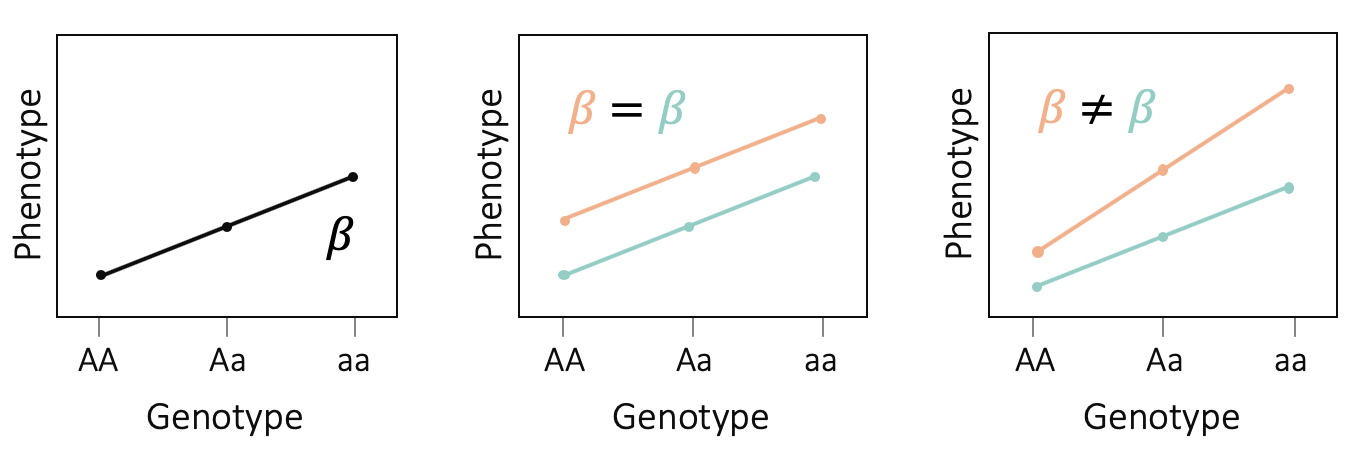
\includegraphics[width=15cm]{Chapter1/Fig/GxE.png}
\caption[\textbf{Illustration of GxE}]{\textbf{Illustration of GxE effect}.\\
a) Genetic effects only. b) Environments have effects on phenotype but do not change the genetic effect. c) Interaction effect between genotype and environment (GxE).}
\label{fig:gxe}
\end{figure}

\subsection{Stratified interaction test}

A possible way to detect interaction effects, is to stratify samples into discrete subgroups based on their environmental exposure.
In e\gls{qtl} mapping, that might for example cluster cells into cell types, or between different conditions.
Then a LM \eqref{eq:Linear_regression_genetics_covariates} or \gls{lmm} (eq. 2.35) is applied to each strata and the marginal variant effects are compared to assess whether there is a significant difference in these effects across the sub-populations.
I will refer to this method as the "stratified interaction test" (ref).

However, as more detailed environmental data is collected, allowing for finer stratification of the population, these methods are no longer optimal as the sub-populations become too small to obtain stable estimates of the variant effects.
For example, as more and more rare cell types are identified and as the definition itself of cell types becomes more blurred, joint analyses become more and more needed. 

\subsection{Single environment interaction test}

A second commonly used method to test for interaction effects is an extension of the LM or \gls{lmm} to include two additional FE terms, an interaction term (GxE) and an environment term (E):

\begin{equation}\label{eq:Interaction_test_FE_LMM}
 \mathbf{y} =  \mathbf{W}\boldsymbol{\alpha} + \mathbf{e}\gamma  + \mathbf{g}\beta_G + \mathbf{e}*\mathbf{g}\beta_{GxE} + \mathbf{u} + \boldsymbol{\psi} 
\end{equation}

Where the test is:

\begin{equation}
 H_{0}: \beta_{GxE}=0 
\end{equation}
vs
\begin{equation}
 H_{1}: \beta_{GxE} \neq 0 
\end{equation}\\

This model allows to directly test for a GxE interaction effect with a certain environment/factor, beyond the additive effects of the SNP and the environment themselves. 
The same model can also be extended to the case of multi-environment interaction by simply adding more environments as FE terms:

\begin{equation}\label{eq:multi_interaction_test_FE_LMM}
 \mathbf{y} =  \mathbf{W}\boldsymbol{\alpha} + \mathbf{e}_1\gamma_1 + \mathbf{e}_2\gamma_2 + ...  + \mathbf{g}\beta_G + \mathbf{e_1}*\mathbf{g}\beta_{GxE,1}+ \mathbf{e_2}*\mathbf{g}\beta_{GxE,2} + .. + \mathbf{u} + \boldsymbol{\psi} 
\end{equation}

However, this becomes quickly unfeasible for large numbers of environments, especially for relatively small sample sizes, because of the dof loss when increasing the number of parameters to estimate (two more for every environment added).


\subsection{StructLMM}

A recently proposed method called StructLMM (structured linear mixed model) allows for the joint analysis of GxE effect of hundreds of environmental variables \cite{moore2019linear} in an efficient manner.
In Chapter 6, I will present an extension to StructLMM for applications to scRNA-seq data so I refer the reader to that chapter for derivations of the updated model.
Instead, I will use this section to give an intuition for the method.\\

The \gls{lmm} in eq. 2.32 models the weight of a given SNP (or effect size, $\beta$) as a scalar, where the assumption is that the effect of a SNP on the trait is the same across all samples.
However, as we have seen, samples belonging to different environmental subgroups can have different effects of a SNP on a trait due to \gls{gxe} \ref{fig:gxe}.
Moreover, the sub-grouping might be extremely complex, possibly driven by several environmental exposures, making adding them all in the model described in eq. 2.39 unfeasible.\\

The intuition of Struct\gls{lmm} is to consider the SNP effect size as split into two components.
The "persistent effect size", which is what we have considered so far, is assumed to be persistent across conditions (I will call this $\beta_G$ from now on). 
The "GxE effect size", on the other hand, is modelled as a random variable and is a Nx1 vector ($\boldsymbol{\beta}_{GxE}$), which depends on the environmental structure of the samples:

\begin{equation}\label{eq:StructLMM-int}
 \mathbf{y} =  \mathbf{W}\boldsymbol{\alpha} + \mathbf{g}\beta_G + \mathbf{g} \otimes \boldsymbol{\beta_{GxE}} + \mathbf{e} + \boldsymbol{\psi} 
\end{equation}

Where $\boldsymbol{\beta_{GxE}} \sim N(\mathbf{0}, \sigma^2_{GxE}\mathbf{E}\mathbf{E}^T)$.\\

The test then is:

\begin{equation}
 H_{0}: \sigma^2_{GxE}=0 
\end{equation}
vs
\begin{equation}
 H_{1}: \sigma^2_{GxE} \neq 0 
\end{equation}\\

StructLMM also allows to test for associations, whilst accounting for GxE effects, essentially testing for any effects, G or GxE.
However, this is beyond the scope of this thesis so I refer the reader to the original paper \cite{moore2019linear}.\\

The main limitation of StructLMM is that for reasons of inference efficiency it does not properly account population sub-structure.
For unrelated individuals, as we discussed in Section 2.3.1, it may be sufficient to include PCs as covariates.
In the case of repeated samples, however, whether it is single cells from the same donor or longitudinal measures from an individual, that is no longer the case.
In Chapter 6, I propose a solution for this problem and apply the model on a variety of simulated and real scRNA-seq data.


% \section{Thesis outline}